%%%%%%%%%%%%%%%%%%%%%%%%%%%%%%%%%%%%%%%%%
% Jacobs Landscape Poster
% LaTeX Template
% Version 1.1 (14/06/14)
%
% Created by:
% Computational Physics and Biophysics Group, Jacobs University
% https://teamwork.jacobs-university.de:8443/confluence/display/CoPandBiG/LaTeX+Poster
% 
% Further modified by:
% Nathaniel Johnston (nathaniel@njohnston.ca)
%
% This template has been downloaded from:
% http://www.LaTeXTemplates.com
%
% License:
% CC BY-NC-SA 3.0 (http://creativecommons.org/licenses/by-nc-sa/3.0/)
%
%%%%%%%%%%%%%%%%%%%%%%%%%%%%%%%%%%%%%%%%%

%----------------------------------------------------------------------------------------
%	PACKAGES AND OTHER DOCUMENT CONFIGURATIONS
%----------------------------------------------------------------------------------------

\documentclass[final]{beamer}

\usepackage[scale=1.24]{beamerposter} % Use the beamerposter package for laying out the poster

\usetheme{confposter} % Use the confposter theme supplied with this template

\definecolor{Mycolor3}{HTML}{FFCC33}
\definecolor{Mycolor2}{HTML}{0C5449}

\setbeamercolor{block title}{fg=ngreen,bg=white} % Colors of the block titles
\setbeamercolor{block body}{fg=black,bg=white} % Colors of the body of blocks
\setbeamercolor{block alerted title}{fg=white,bg=Mycolor2!70} % Colors of the highlighted block titles
\setbeamercolor{block alerted body}{fg=black,bg=Mycolor2!10} % Colors of the body of highlighted blocks
% Many more colors are available for use in beamerthemeconfposter.sty

%-----------------------------------------------------------
% Define the column widths and overall poster size
% To set effective sepwid, onecolwid and twocolwid values, first choose how many columns you want and how much separation you want between columns
% In this template, the separation width chosen is 0.024 of the paper width and a 4-column layout
% onecolwid should therefore be (1-(# of columns+1)*sepwid)/# of columns e.g. (1-(4+1)*0.024)/4 = 0.22
% Set twocolwid to be (2*onecolwid)+sepwid = 0.464
% Set threecolwid to be (3*onecolwid)+2*sepwid = 0.708

\newlength{\sepwid}
\newlength{\onecolwid}
\newlength{\twocolwid}
\newlength{\threecolwid}
\setlength{\paperwidth}{48in} % A0 width: 46.8in
\setlength{\paperheight}{36in} % A0 height: 33.1in
\setlength{\sepwid}{0.024\paperwidth} % Separation width (white space) between columns
\setlength{\onecolwid}{0.22\paperwidth} % Width of one column
\setlength{\twocolwid}{0.464\paperwidth} % Width of two columns
\setlength{\threecolwid}{0.708\paperwidth} % Width of three columns
\setlength{\topmargin}{-0.5in} % Reduce the top margin size
%-----------------------------------------------------------

\usepackage{graphicx}  % Required for including images

\usepackage{multirow}

\usepackage{booktabs} % Top and bottom rules for tables


\usepackage{tikz}
\usetikzlibrary{matrix}

\usetikzlibrary{shapes.misc}
\usetikzlibrary{fadings,shapes.arrows,shadows}   

\tikzfading[name=arrowfading, top color=transparent!0, bottom color=transparent!95]
\tikzset{arrowfill/.style={top color=black!5, bottom color=black!40, general shadow={fill=black, shadow yshift=-0.8ex, path fading=arrowfading}}}
\tikzset{arrowstyle/.style={draw=black	,arrowfill, single arrow,minimum height=#1, single arrow,
single arrow head extend=.4cm,}}

\newcommand{\tikzfancyarrow}[2][2cm]{\tikz[baseline=-0.5ex]\node [arrowstyle=#1] {#2};}

\tikzset{cross/.style={cross out, draw=black, minimum size=2*(#1-\pgflinewidth), inner sep=0pt, outer sep=0pt},
%default radius will be 1pt. 
cross/.default={1pt}}


%----------------------------------------------------------------------------------------
%	TITLE SECTION 
%----------------------------------------------------------------------------------------

\title{Sequential Query Expansion using Concept Graph} % Poster title

\author{  Saeid Balaneshin-kordan and
 Alexander Kotov} % Author(s)

\institute{Computer Science Department, Wayne State University} % Institution(s)

%----------------------------------------------------------------------------------------

\begin{document}

\addtobeamertemplate{block end}{}{\vspace*{2ex}} % White space under blocks
\addtobeamertemplate{block alerted end}{}{\vspace*{2ex}} % White space under highlighted (alert) blocks

\setlength{\belowcaptionskip}{2ex} % White space under figures
\setlength\belowdisplayshortskip{2ex} % White space under equations

\begin{frame}[t] % The whole poster is enclosed in one beamer frame

\begin{columns}[t] % The whole poster consists of three major columns, the second of which is split into two columns twice - the [t] option aligns each column's content to the top

\begin{column}{\sepwid}\end{column} % Empty spacer column

\begin{column}{\onecolwid} % The first column

%----------------------------------------------------------------------------------------
%	OBJECTIVES
%----------------------------------------------------------------------------------------

\begin{alertblock}{Objectives}
\begin{itemize}
\item To discover \textbf{effective latent concepts} for query
expansion from from manually and automatically constructed concept graphs (or semantic networks), in which the nodes correspond to words
or phrases and the typed edges designate semantic relationships between words and phrases. 
\item To leverage \textbf{large and dense concept graphs}, in which the number of candidate concepts that
are related to query terms and phrases and need to be examined increases exponentially with the distance from the
original query concepts.
\end{itemize} 
\end{alertblock}

%----------------------------------------------------------------------------------------
%	INTRODUCTION
%----------------------------------------------------------------------------------------

\begin{block}{Optimization Problem}

\begin{itemize}
\item \textcolor{red}{\textbf{Objective Function:}} total number of \textbf{evaluated} concepts 

\item \textcolor{red}{\textbf{Constraint:}}
precision of retrieval results


\begin{align*}\label{eq:opt}
\min_{\mathbb{\tilde C}_{k}^{ut}}\quad&\bigg\{\sum_{i=1}^k{N_i}\bigg\}\nonumber\\
\text{s.t.}\quad& E(\mathbb{\tilde R}_\Lambda;\mathbb{T})>\theta_Q\ ,
\end{align*}
\end{itemize}
\end{block}



\begin{block}{Approximate Solution} 
\begin{enumerate}
\item The candidate
concepts are \textbf{sorted} using  computationally \textbf{inexpensive features}.

\item This sorting is utilized in the \textbf{second stage} to sequentially \textbf{select expansion concepts} by using computationally \textbf{expensive
features}.

\end{enumerate}

\begin{table}[htb!]
\label{tabl: 3regions_}
\centering
\begin{tabular}{@{}lll@{}}
\toprule
\textbf{Criterion}                                                          &  & \textbf{Decision}              \\ \midrule
\multirow{3}{*}{If ${\color{red}\tilde Q_r(C_{(i,j)})}\ge\beta_U$}          &  & Select concept $C_{(i,j)}$ \&  \\
                                                                            &  & Continue with the same         \\
                                                                            &  & concept layer                  \\ \midrule
\multirow{3}{*}{If $\beta_L\le {\color{red}\tilde Q_r(C_{(i,j)})}<\beta_U$} &  & Discard concept $C_{(i,j)}$ \& \\
                                                                            &  & Continue with the same         \\
                                                                            &  & concept layer                  \\ \midrule
\multirow{3}{*}{If ${\color{red}\tilde Q_r(C_{(i,j)})}<\beta_L$}            &  & Discard concept $C_{(i,j)}$ \& \\
                                                                            &  & Move to the next               \\
                                                                            &  & concept layer                  \\ \bottomrule
\end{tabular}
\end{table}
\end{block}

%------------------------------------------------



%----------------------------------------------------------------------------------------

\end{column} % End of the first column

\begin{column}{\sepwid}\end{column} % Empty spacer column

\begin{column}{\twocolwid} % Begin a column which is two columns wide (column 2)

\setbeamercolor{block alerted body}{fg=black,bg=white} % Change the alert block body colors

\begin{alertblock}{Concept Graph for Query: \textcolor{yellow}{\Large poach wildlife preserve}}

\newsavebox{\conceptgraphitems}
\sbox{\conceptgraphitems}{
\parbox{\textwidth}{
\begin{figure}[htb!]
 \centering
 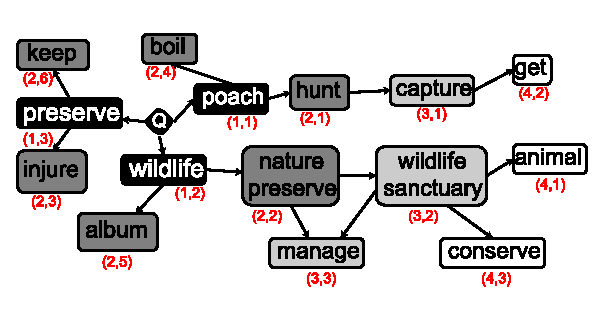
\includegraphics[scale=4]{images/conceptGraph2.eps}
 \label{fig:layers}
\end{figure}
\begin{itemize}
\item Concept Graph: \textcolor{red}{ConceptNet 5} 
\item The $1^\text{st}$ number in parentheses: concept layer,
the $2^\text{nd}$ number: index of a concept in the concept layer. 
\end{itemize}

}}

\begin{tikzpicture}
\node [shape=rectangle, scale=1]  at (0,0)  {\usebox{\conceptgraphitems}}
;

\draw[red, fill=red, fill opacity=0.03] (-9.5,5.5) ellipse (50pt and 50pt);

\draw[red, fill=red, fill opacity=0.03] (-10,5.5) ellipse (270pt and 120pt);

\draw[red, fill=red, fill opacity=0.03] (-9.5,5.5) ellipse (400pt and 210pt);

\draw[red, fill=red, fill opacity=0.03] (-6.5,5.5) ellipse (520pt and 260pt);

\draw[red, fill=red, fill opacity=0.03] (-1,5.5) ellipse (700pt and 300pt);

\end{tikzpicture}
\end{alertblock}

\begin{alertblock}{Proposed Sequential Concept Selection}

\newsavebox{\speciesone}
\sbox{\speciesone}{
\begin{tabular}{|l|l|}
\hline
\textbf{Decision} & \textbf{Criterion} \\\hline
\colorbox{green!20}{Select concept \&} & \multirow{2}{*}{\colorbox{green!20}{$\tilde Q_r(C_{(i,j)})\ge\beta_U$}}\\
\colorbox{green!20}{continue} & \\
\hline
\colorbox{blue!20}{Discard concept \&} & \multirow{2}{*}{\colorbox{blue!20}{$\beta_L\le \tilde Q_r(C_{(i,j)})<\beta_U$}}\\
\colorbox{blue!20}{continue} &\\
\hline
\colorbox{red!20}{Discard concept  \&} & \multirow{2}{*}{\colorbox{red!20}{$\tilde Q_r(C_{(i,j)})<\beta_L$}}\\
\colorbox{red!20}{move to next layer}& \\
\hline
\end{tabular}
  }

\noindent 
\begin{tikzpicture}
\draw[white] (-29,0) -- (-42.1,0) -- (-42.1,35) -- (-29,35) -- (-29,0);

\node[anchor=south west,inner sep=0] at (-30,22) {
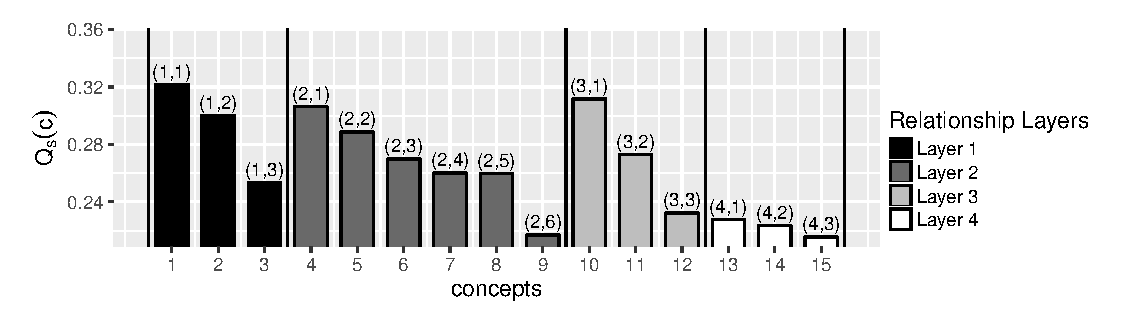
\includegraphics[width=0.7\textwidth]{images/SNOPC_stepI.eps}
};
\node[anchor=south west,inner sep=0] at (-40,27) {Stage I:};
\node[anchor=south west,inner sep=0] at (-41,26) {\scriptsize Initial Concept Sorting};


\node [shape=rectangle]  at (-38.1,16.2)   {Stage II:};
\node [shape=rectangle]  at (-38.1,14.8)   {\scriptsize - Sort Concepts at Each Layer};
\node [shape=rectangle]  at (-38.1,13.8)   {\scriptsize according to $\tilde Q_s(C_{(i,j)})$};
\node[anchor=south west,inner sep=0] at (-42.6,12.4) {\scriptsize - Sequential Concept Selection};

\node[anchor=south west,inner sep=0] at (-30,9.5) {
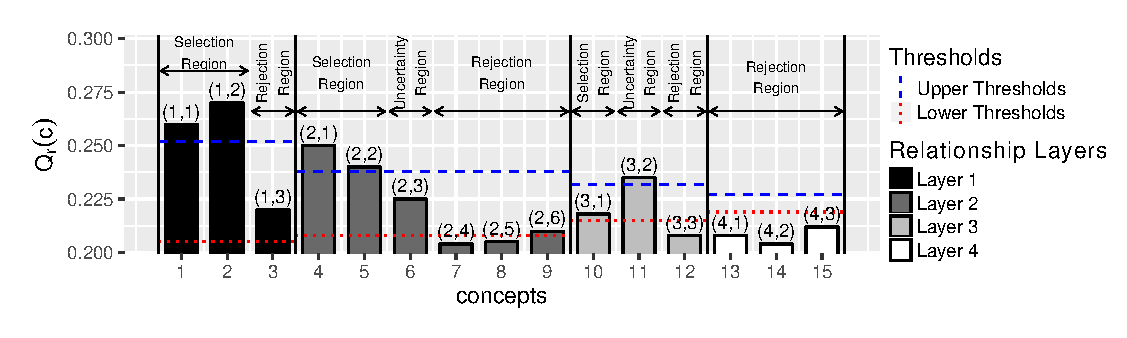
\includegraphics[width=0.7\textwidth]{images/SNOPC_stepII.eps}
};


% circles:

\draw[green, fill=green, fill opacity=0.4] (-24.10,16.37) circle (30pt);


\draw[green, fill=green, fill opacity=0.4] (-22.60,17.35) circle (30pt);

\draw[blue, fill=blue, fill opacity=0.4] (-20.90,14.05) circle (30pt);

\draw[green, fill=green, fill opacity=0.4] (-19.20,16.05) circle (30pt);

\draw[green, fill=green, fill opacity=0.4] (-17.65,15.05) circle (30pt);

\draw[blue, fill=blue, fill opacity=0.4] (-16.10,14.30) circle (30pt);

\draw[red, fill=red, fill opacity=0.4] (-14.55,12.70) circle (30pt);

\draw[red, fill=red, fill opacity=0.4] (-13.00,12.70) circle (30pt);

\draw[red, fill=red, fill opacity=0.4] (-11.45,12.70) circle (30pt);

\draw[blue, fill=blue, fill opacity=0.4] (-9.75,13.70) circle (30pt);

\draw[green, fill=green, fill opacity=0.4] (-8.10,14.70) circle (30pt);

\draw[red, fill=red, fill opacity=0.4] (-6.50,12.60) circle (30pt);

\draw[red, fill=red, fill opacity=0.4] (-4.80,12.60) circle (30pt);

\draw[red, fill=red, fill opacity=0.4] (-3.10,12.60) circle (30pt);

\draw[red, fill=red, fill opacity=0.4] (-1.50,12.60) circle (30pt);

% decisions

\node [shape=rectangle, scale=0.5]  at (-37.1,4)  {\usebox{\speciesone}};


% actions

\node [arrowstyle=40pt, scale=1]at (-25.00,3) {Actions};


\node [shape=rectangle, scale=1, fill=white]  at (-15.1,4.5)   {\textbf{Continue}};


\node [shape=rectangle, scale=1, fill=white]  at (-15.1,6.5)   {$\quad$\textbf{Select}$\quad$};


\node [shape=rectangle, scale=1, fill=white]  at (-15.1,2.5)   {\textbf{Discard}};


\node [shape=rectangle, scale=1, fill=white]  at (-15.1,0.5)   {$\quad$\textbf{STOP}$\quad$};


\node [shape=rectangle, scale=1, fill=white,text width=400pt]  at (-0.0,4.00)   {Number of Evaluated Concepts: 11 (26\% less)};



\end{tikzpicture}

\end{alertblock}

\begin{columns}[t,totalwidth=\twocolwid] % Split up the two columns wide column

\begin{column}{\onecolwid}\vspace{-.6in} % The first column within column 2 (column 2.1)

%----------------------------------------------------------------------------------------
%	MATERIALS
%----------------------------------------------------------------------------------------


%----------------------------------------------------------------------------------------

\end{column} % End of column 2.1

\begin{column}{\onecolwid}\vspace{-.6in} % The second column within column 2 (column 2.2)

%----------------------------------------------------------------------------------------
%	METHODS
%----------------------------------------------------------------------------------------



%----------------------------------------------------------------------------------------

\end{column} % End of column 2.2

\end{columns} % End of the split of column 2 - any content after this will now take up 2 columns width

%----------------------------------------------------------------------------------------
%	IMPORTANT RESULT
%----------------------------------------------------------------------------------------



\begin{alertblock}{Important Result}



\end{alertblock} 

%----------------------------------------------------------------------------------------

\begin{columns}[t,totalwidth=\twocolwid] % Split up the two columns wide column again

\begin{column}{\onecolwid} % The first column within column 2 (column 2.1)

%----------------------------------------------------------------------------------------
%	MATHEMATICAL SECTION
%----------------------------------------------------------------------------------------



%----------------------------------------------------------------------------------------

\end{column} % End of column 2.1

\begin{column}{\onecolwid} % The second column within column 2 (column 2.2)

%----------------------------------------------------------------------------------------
%	RESULTS
%----------------------------------------------------------------------------------------

%----------------------------------------------------------------------------------------

\end{column} % End of column 2.2

\end{columns} % End of the split of column 2

\end{column} % End of the second column

\begin{column}{\sepwid}\end{column} % Empty spacer column

\begin{column}{\onecolwid} % The third column

\begin{figure}
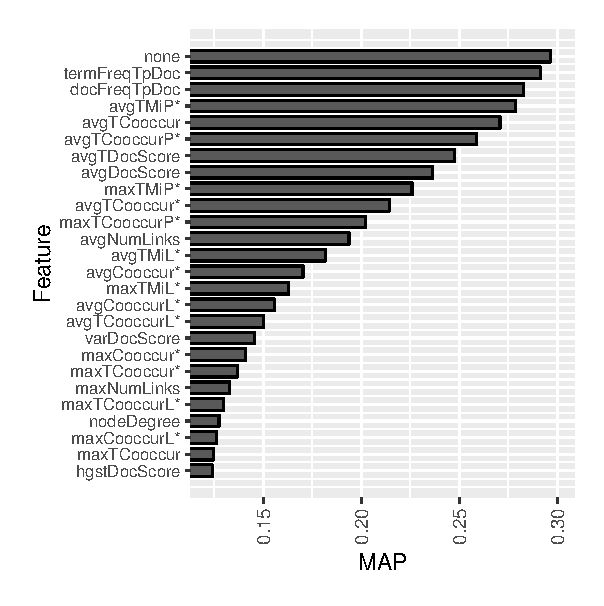
\includegraphics[width=0.9\linewidth]{images/featuresSorted.eps}
\caption{Feature Ablation}
\end{figure}

%----------------------------------------------------------------------------------------
%	CONCLUSION
%----------------------------------------------------------------------------------------

\begin{block}{Conclusion}

The main contribution of this work is a two-stage method
for sequential selection of effective concepts for query expansion from the concept graph. The proposed method is formulated as an optimization problem with the goal of evaluating the least possible number of candidate concepts needed
to ensure a given precision of retrieval results. 

\end{block}

%----------------------------------------------------------------------------------------
%	ADDITIONAL INFORMATION
%----------------------------------------------------------------------------------------

%----------------------------------------------------------------------------------------
%	REFERENCES
%----------------------------------------------------------------------------------------

\begin{block}{References}

\nocite{*} % Insert publications even if they are not cited in the poster
\small{\bibliographystyle{unsrt}
\bibliography{sample}\vspace{0.75in}}

\end{block}

%----------------------------------------------------------------------------------------
%	ACKNOWLEDGEMENTS
%----------------------------------------------------------------------------------------

\setbeamercolor{block title}{fg=red,bg=white} % Change the block title color

%----------------------------------------------------------------------------------------
%	CONTACT INFORMATION
%----------------------------------------------------------------------------------------


\setbeamercolor{block alerted title}{fg=black,bg=Mycolor3} % Change the alert block title colors
\setbeamercolor{block alerted body}{fg=black,bg=white} % Change the alert block body colors

\begin{alertblock}{Contact Information}

\begin{itemize}
\item Web: \href{http://www.balaneshin.com/}{http://www.balaneshin.com/}
\item Email: \href{mailto:saeid@wayne.edu}{saeid@wayne.edu}
\item Phone: +1 (313) 316 6723
\end{itemize}

\end{alertblock}

\begin{center}
\begin{tabular}{ccc}

\includegraphics[width=0.3\linewidth]{images/warrior_banded_logo.jpg} & \hfill & 
\includegraphics[width=0.3\linewidth]{images/cikm16.png}
\end{tabular}
\end{center}

%----------------------------------------------------------------------------------------

\end{column} % End of the third column

\end{columns} % End of all the columns in the poster

\end{frame} % End of the enclosing frame

\end{document}
